% Chapter Template

\chapter{Discussion} % Main chapter title

\label{Chapter7} % Change X to a consecutive number; for referencing this chapter elsewhere, use \ref{ChapterX}

%----------------------------------------------------------------------------------------
%	SECTION 1
%----------------------------------------------------------------------------------------

\section{Whole Proof Generation}
\label{wholeproof}

We were quite surprised to find out that performance on mobile ARM processors is almost as good as x86-64 i7 performance. Performance on the i7 processor is a bit better, however, ARM's 8 cores and higher price tag make the performance gap really narrow.\\
\\
Another interesting insight is the importance of the processor word width. 32-bit code was slower than its 64-bit counterpart on both architectures. This performance penalty is incurred because of arithmetic operations. zk-SNARKs rely on 381-bit finite prime field arithmetic. Emulating these operations requires fewer 64-bit than 32-bit operations. For 32-bit code every 64-bit addition needs to be decomposed into 2 32-bit additions. Every multiplication requires 3 32-bit multiplications (4 if we want to keep the high bits). On top of this, there are several ADD instructions needed to compute the final product (Figure \ref{fig:mulcomp}).\\
\begin{figure}[h]
    \centering
    \begin{minipage}[t]{0.45\linewidth}
        \begin{lstlisting}[basicstyle=\small,language={[x86masm]Assembler}]
push  esi
mov   ecx, dword ptr [esp + 16]
mov   esi, dword ptr [esp + 8]
mov   eax, ecx
imul  ecx, dword ptr [esp + 12]
mul   esi
imul  esi, dword ptr [esp + 20]
add   edx, ecx
add   edx, esi
pop   esi
ret
        \end{lstlisting}
        \end{minipage}%
        \hfill\vrule\hfill
        \begin{minipage}[t]{0.45\linewidth}
        \begin{lstlisting}[basicstyle=\small,language={[x64]Assembler}]
mov   rax, rdi
imul  rax, rsi
ret
        \end{lstlisting}
        \end{minipage}

        \caption{Assembly of the function that multiplies two 64-bit numbers on x86 (left) and x64 (right)}
        \label{fig:mulcomp}
\end{figure}
\\
The stress test showed that phones are prone to overheat, and throttle the computation of proofs if under heavy load. This happens after several proofs have been computed, even if nothing else is running on the device. Laptops don't show this behavior due to the fans disperse the heat. Note that the test was performed on a laptop with GPU turned off.

\section{FFT and Multiexp}

The results of this test showed no surprising facts. Multiexponentiation and FFT are the most time-consuming parts of zk-SNARKs. Parallelizing FFT would lead to minimal performance gains due to it taking only 15\% of execution time. Considering that the simplified Pippenger's algorithm used for multiexponentiation is inherently parallelizable, it lent itself as the perfect candidate for GPU acceleration.

\section{131k Test}

Integrated GPUs performed poorly when compared to CPUs and discrete GPUs. This rules out the use of mobile GPUs for accelerating zk-SNARKs. If we take a look at frequencies and core counts of discrete and integrated GPUs, it is clear that Intel and Mali GPUs will be at least an order of magnitude slower than NVIDIA and AMD cards. The actual surprise is that not even discrete GPUs can beat CPUs running Pippenger's algorithm. In this section, we explain multiple contributing factors.\\
\\
\subsection{Processor Word Length - 32 vs 64}

As we concluded in Section \ref{wholeproof}, processor word length plays an important role in zk-SNARK performance. With GPUs, this effect is further amplified by the memory hierarchy. All of today's GPUs are still clusters of 32-bit RISC cores operating in unison \cite{nvidiapascalinstructions, amdpolarisinstructions}. Small word length means that these cores need to execute several times more instructions than CPUs running equivalent code. It is interesting to note that GPUs are optimized towards floating-point numbers, leading to lower throughput for integer operations \cite{nvidiathroughput}.\\

\subsection{Branch Divergence}

A common problem with code running on GPUs is branch divergence. When CPU encounters a branch in the code, it will execute only one of two code paths. Unfortunately, all GPU cores in a group need to execute the same instruction. To satisfy this, GPUs will execute both branches, and tell cores to ignore the instructions which don't satisfy their condition check.\\
\\
However, profiling on our AMD card showed thread convergence rate of 85\%. Improving this further would lead to minimal gains in performance.

\subsection{Inlining, Loops and Constants}

While functions are considered good practice on CPUs, using them on GPUs can significantly hinder performance. Function calls require a call stack. Unfortunately, this stack is stored in global memory. For small kernels, this isn't a problem because the stack can be cached. However, our kernels have elliptic curve points as arguments, so the stack is too big to fit in the cache. Another problem is that Pippenger's algorithm requires an array of elliptic curve points with random access \cite{nvidiaarrayindexing}. Kernel disassembly of NVIDIA code showed that these arrays are stored on the stack (i.e. in global memory).\\
\\
Inlining function calls and unwrapping loops reduces divergence and removes the stack. However, it substantially increases the size of the code. This, combined with 32-bit registers, results in code that is too large to fit in the instruction cache, incurring a performance penalty. Analysis of AMD disasembly shows that the kernels were around 90 KB in size, while the instruction cache has only 30 KB \cite{amdgcnarch}. On the other hand, NVIDIA compiler actively tried to prevent code explosion by keeping some functions intact, even though they had been marked inline. Unfortunately, this resulted in an enormous call stack.\\
\\
OpenCL uses global memory to store constants. Usually, they can be cached, so the performance penalty doesn't need to be high. However, if the kernel has a lot of memory traffic, constants will be pushed out of the cache and will be fetched every time they are used. To prevent this, we used macros in place of variables, hoping that compilers will use immediate load instructions instead of memory reads. Unfortunately, both NVIDIA and AMD compilers detected constants and put them in global memory.

\begin{figure}[h]
    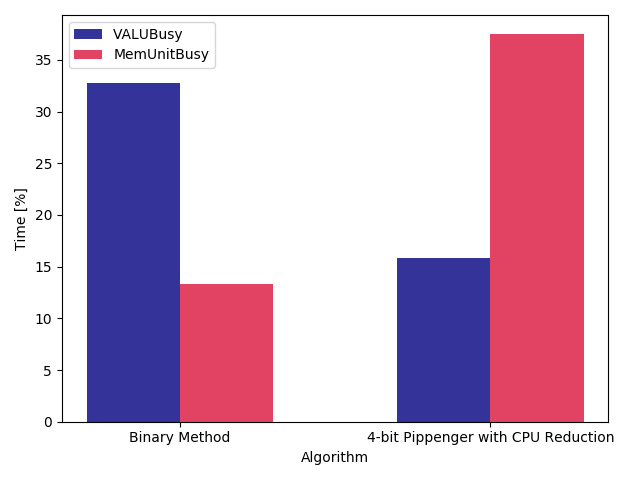
\includegraphics[width=\linewidth]{Figures/profiler.png}
    \caption{Memory and ALU Activity of Binary Method and 4-bit Pippenger with CPU Reduction Running on AMD RX 580}
    \label{fig:profiler}
\end{figure}

All of these things, combined with high register usage of kernels (more than 160 registers on NVIDIA, 256 on AMD), results in high memory traffic and low occupancy for Pippenger's algorithm on GPUs. Figure \ref{fig:profiler} shows data from AMD profiler - vector ALU and memory unit usage for the binary method and Pippenger's algorithm. Even though Pippenger's algorithm is faster, it barely uses ALU, compared to memory. CPUs can run the same algorithm with much larger array sizes without incurring a performance penalty, leading to better performance.

\subsection{Performance Gains}

It is possible to attain a speed-up of 25-30\% by running CPU and GPU together and distributing work between them. This scheme would involve putting (a smaller) part of the exponent on GPU, exponentiating the rest on CPU, and combining the results. Unfortunately, due to different ratio's of CPU and GPU power, we would need to maintain either a table for most common combinations or run a test once to determine the optimal ratio.\\
\\
However, the gains are minimal even with more powerful GPUs. Graphic cards draw a lot of power, heat up the machine and increase fan noise. This scheme would require us to maintain two versions of the same code and would be economical only if we already own a strong GPU. If we want to buy a machine specifically for zCash, it would be more economical to buy a processor with more cores.